\chapter{Empirical Experiments}\label{chapter:experiments}
% \setcounter{page}{0}
% \pagenumbering{arabic}

\section{Prices and Filling Information}
To have a comprehensive understanding of how trades in trade book correspond to orders in order book, Figure~\ref{fig:p_f_i} provides an overview of the whole active trading hours from 10:00 am to 4:00 pm on 31st January. It shows how filled price in the trade book track the mid-price in the order book, the distribution of passive and aggressive trades, and the spread range for each trade. The lower subplot presents the filled volume for each trading record.
\begin{figure}[h]
    \centering
    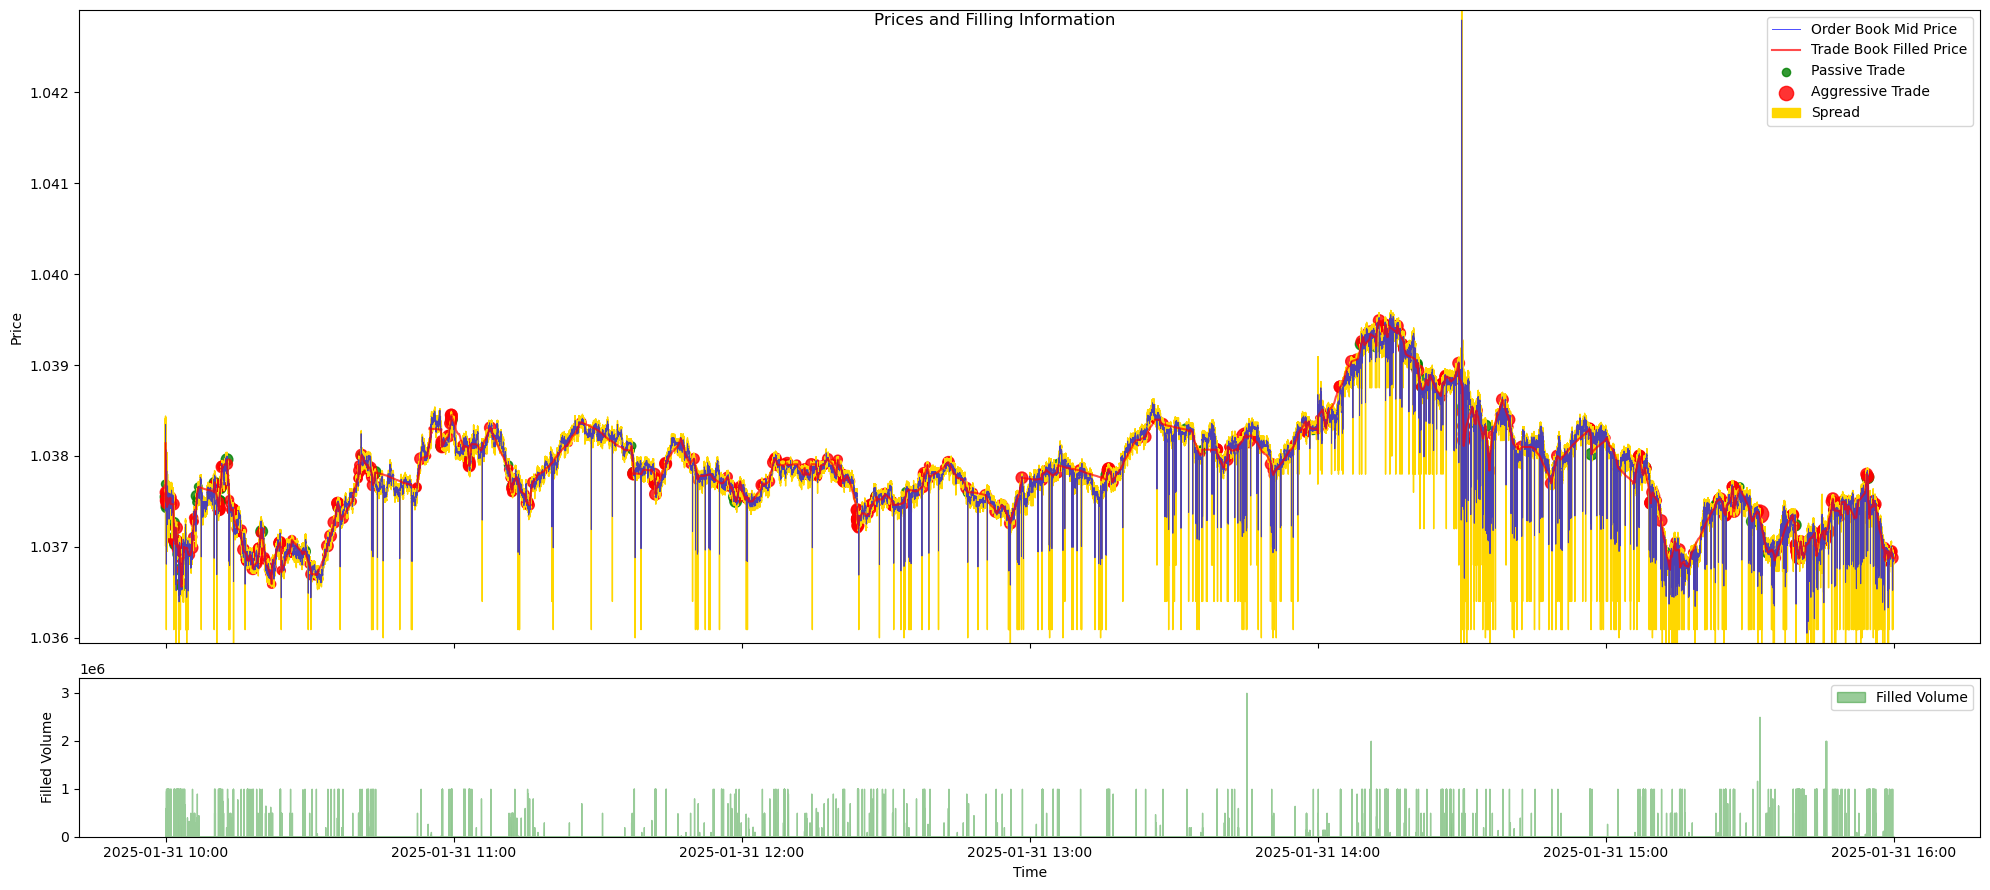
\includegraphics[width=1\linewidth]{figures/Prices and Filling Information.png}
    \caption{Prices and filling information. This plot shows the mid-price from the order book (blue line), trade book filled prices (red line), and spread (yellow shading). Passive trades (green dots) and aggressive trades (red dots) are highlighted. The bottom panel represents the filled volume over time.}
    \label{fig:p_f_i}
\end{figure}
As can be seen in Figure~\ref{fig:p_f_i}, the mid-price has the highest point between 14:00 and 15:00. The filled price fits the mid-price well. We can see there are a lot of red dots which shows that they are aggressive trades. We didn't classify bid or ask side because it's not the research target in the thesis. These aggressive trades go outside the spread range. The size of dots stands for relative volume of the trades. In other words, when the volume is large compared to other timestamps, the size of the dot will be larger. Therefore, we can easily see the active trading time point in the plot. Moreover, red dots represent aggressive trades in the trade book. We can see the red dots are more than green ones, which indicates that a lot of orders get filled by aggressive traders taking out them of the order book, instead of passively waiting for the market movements. This aligns with our need to improve the backtesting environment by predicting aggressive trades across the order book. Specially, there are several sparks in the trend of mid-price in the order book. These are caused by...

From the bottom panel, in the beginning of 10:00, 15:45, 14:11, there are high volume up to 2,000,000, which are higher than common volume 1,000,000. At 13:45, the highest trading volume occurs as 3,000,000. Combined the two plots together, we can see when there's a drop, it's often accompanied by many trading records or large trades. 

\begin{figure}[h]
    \centering
    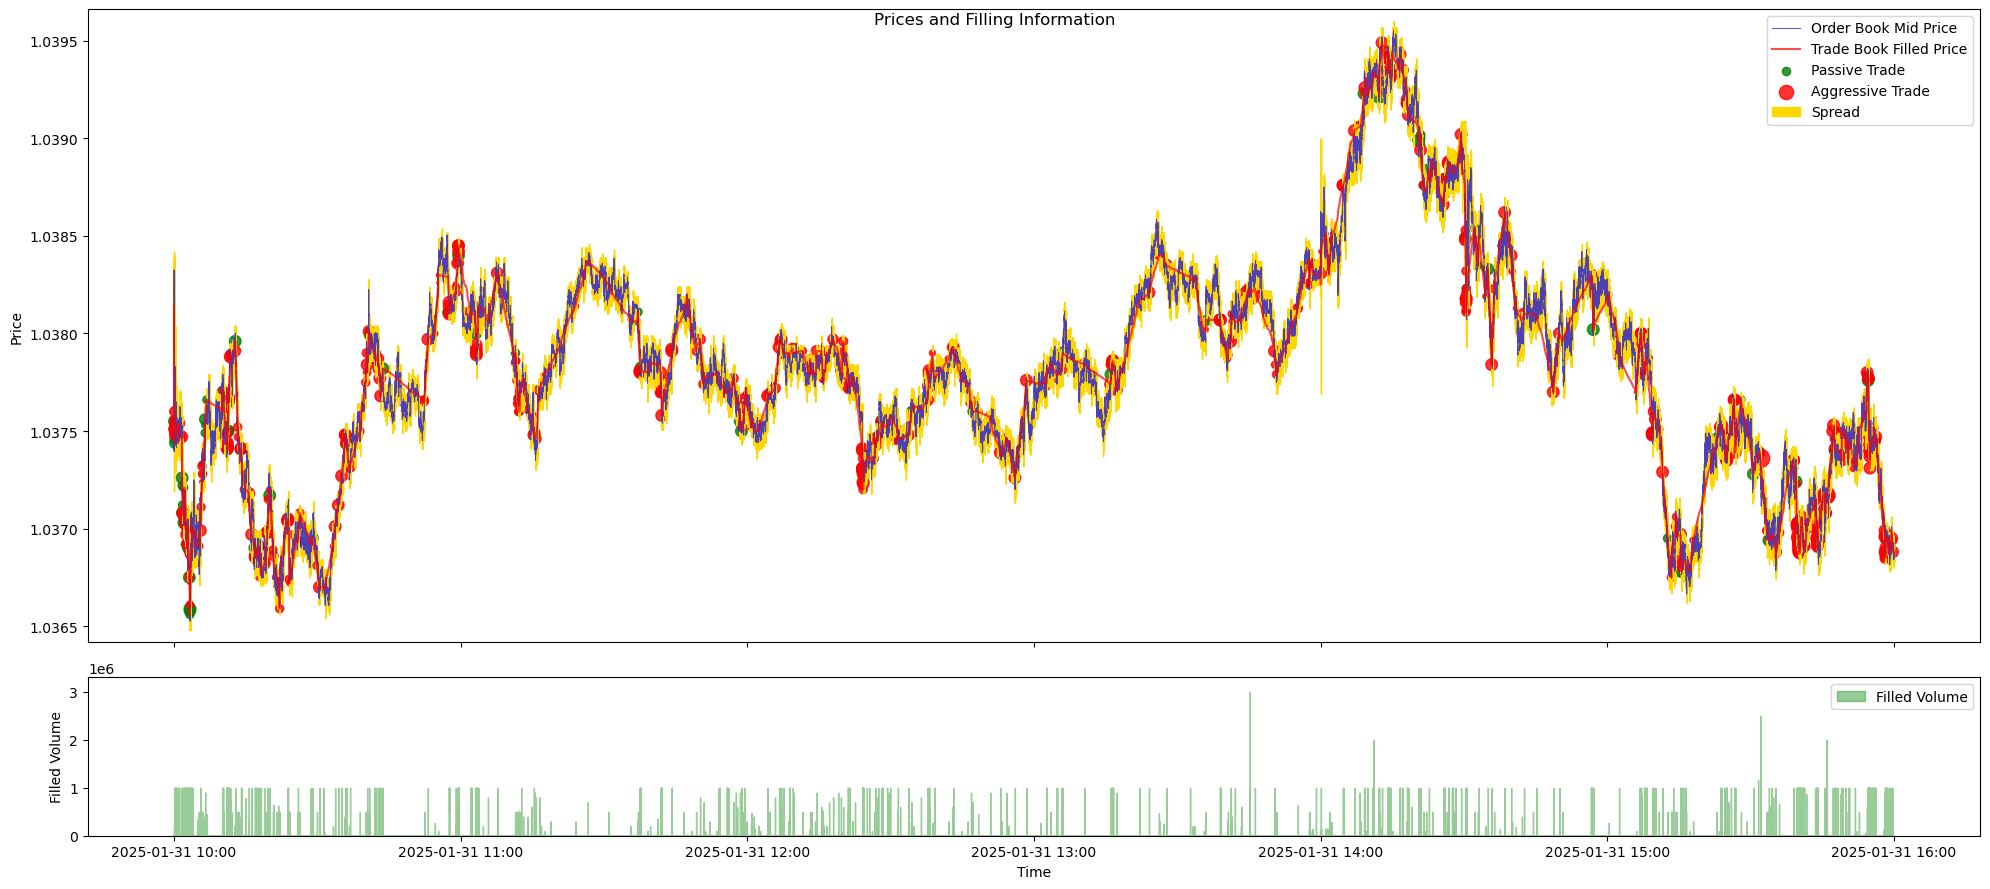
\includegraphics[width=1\linewidth]{figures/Filtered Prices and Filling Information.png}
    \caption{Filtered prices and filling information. Similar to Figure~\ref{fig:p_f_i}, but filtering sharp jump points. The price and trade dynamics remain the same, without increased variability for better general trend capture}
    \label{fig:f_p_f_i}
\end{figure}

In the Figure~\ref{fig:f_p_f_i} after filtering 1,232 sparks in the data, we can clearly see some clustering for both passive and aggressive trades. For example, in the beginning of 10:00, many passive trades gather here. It may because there's a sharp dropping movement in the market, many limit orders are filled. Furthermore, many aggressive trades gather around  


% Evaluating how well the model captures aggressive trades movements and distribution.
% Market realism (stylized facts: price impact, spread, volume clustering).
\section{Step-by-Step Prediction Results}
The prediction framework consists of three sequential stages. The first stage employs an XGBoost model to identify potential aggressive trade timestamps while reducing the overall dataset size. The second stage is GRU networks. It serves as a bridge between machine learning approaches and stochastic processes, centering around potential timestamps where trades could happen from XGBoost to improve the class balance and generate high-confidence timestamps likely to contain aggressive trades. The final stage implements a tailored Hawkes process that estimates event intensity while incorporating MN's specific trading information. In the end this multi-stage approach produces a detailed and interpretable set of predictions for potential aggressive trading events.

We present the prediction results of each stage using a representative trading day. The training dataset consists of the whole trading day from January 31, 2025, 10:00:00 to 15:59:59 PM, containing 307,764 rows. The testing dataset is a 30-minute window from January 30, 2025, 09:08:57 to 09:38:51, with 18,848 rows. This specific time window was selected as it represents a commonly used timeframe for FX trading backtesting within the MN platform.

\subsection{XGBoost Stage: With and Without KMeansSMOTE}
KMeansSMOTE, introduced in the Methodology chapter, is an oversampling technique designed to address class imbalance in training data. We compare the XGBoost prediction results with and without KMeansSMOTE to evaluate the influence of oversampling. The impact of applying this oversampling method on both class balance and prediction quality is analyzed.

We first present the classification results of XGBoost trained with KMeansSMOTE. The KMeansSMOTE configuration is as follows:

\begin{verbatim}
pipeline = Pipeline([
("imputer", SimpleImputer(strategy="median")),
("smote", KMeansSMOTE(random_state=42,
cluster_balance_threshold=0.002,
kmeans_estimator=KMeans(n_clusters=200, random_state=42),
sampling_strategy=0.5))
])
\end{verbatim}

The median strategy fills missing values with the median of each feature. A cluster balance threshold of 0.02 ensures oversampling is done in 'safe' areas where there are at least some genuine minority examples. This can improve sample quality and reducing class overlap or overfitting risks. As a result, the training set has equal amounts of class 1 and class 0, but most class 1 samples are artificially created by oversampling.

%from here start
As shown in Figure~\ref{fig:xgb-pred-vs-true-km}, the model catches many true positives. The class balancing done by KMeansSMOTE reduces the bias toward class 0 and helps the model learn better from the underrepresented class 1.

Table~\ref{tab:xgb-confusion-km} shows the confusion matrix. There are 11,545 test samples after filtering. Among them, 11,487 are predicted as class 0 (no trade), and only 58 are predicted as class 1 (trade). The model correctly finds 39 true positives and 7,293 true negatives. The dataset size drops from 18,848 to 11,545 rows, which is 38.75\% of the original. This helps improve speed and keeps most of the important trade points.

Moreover, Table~\ref{tab:xgb-classification-report-km} shows the detailed classification report. We mainly care about the prediction performance for class 1, since this is the main goal of the whole research. The precision of class 0 is not meaningful here because the original data is extremely imbalanced. Although the precision for class 1 is still very low at 0.0034, the recall reaches 0.5735. This means the model finds more true trades, even though oversampling brings some noise. This makes preparation for next GRU networks to train around aggressive trades timestamps. The F1-score for class 1 is 0.0067, but this result already gives a good starting point for the next filtering stages.


\begin{figure}[H]
    \centering
    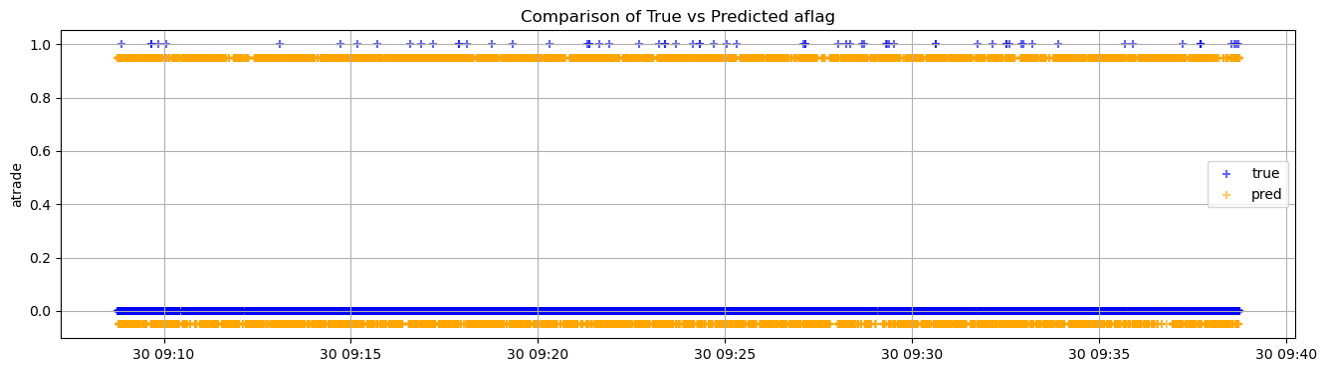
\includegraphics[width=\textwidth]{figures/XGBoost comparison1.png}
    \caption{Comparison of true vs. predicted $\bar{\alpha}$ from XGBoost with KMeansSMOTE. 
    The blue '+' markers show the true class labels, and the orange '+' markers show the predicted ones. To make the plot easier to read, the predicted values are moved down by 0.05 on the y-axis. This small shift helps to see clearly how well the predictions match the true labels.
    }
    \label{fig:xgb-pred-vs-true-km}
\end{figure}

\begin{table}[H]
    \centering
    \caption{Confusion matrix of XGBoost with KMeansSMOTE}
    \label{tab:xgb-confusion-km}
    \begin{tabular}{lcc}
        \toprule
        & Predicted 0 & Predicted 1 \\
        \midrule
        True 0 & 7,293 & 11,487 \\
        True 1 & 29 & 39 \\
        \bottomrule
    \end{tabular}
\end{table}
\begin{table}[H]
    \centering
    \caption{Classification report of XGBoost with KMeansSMOTE}
    \label{tab:xgb-classification-report-km}
    \begin{tabular}{lcccc}
        \toprule
        Class & Precision & Recall & F1-score & Support \\
        \midrule
        0 & 0.9962 & 0.3882 & 0.5587 & 18780 \\
        1 & 0.0035 & 0.5882 & 0.0069 & 68 \\
        \midrule
        Accuracy & \multicolumn{4}{c}{0.3890} \\
        Macro avg & 0.4998 & 0.4882 & 0.2828 & 18848 \\
        Weighted avg & 0.9926 & 0.3889 & 0.5567 & 18848 \\
        \bottomrule
    \end{tabular}
\end{table}

Without KMeansSMOTE, even if we reach the same recall, the precision is even worse (only 0.0019). That means almost all predicted class 1 are wrong. The F1-score is just 0.0038, which is only half of the score from XGBoost with KMeansSMOTE. Also, the filter effect is weaker. More lines (12,479) are left in the result, which makes the next detection step slower and more difficult. So using KMeansSMOTE helps not only improve model performance but also makes the pipeline more efficient.

\begin{table}[H]
    \centering
    \caption{Confusion matrix of XGBoost without KMeansSMOTE}
    \label{tab:xgb-noKM}
    \begin{tabular}{lccc}
        \toprule
        Class & Precision & Recall & F1-score\\
        \midrule
        1 & 0.0019 & 0.5881 & 0.0038 \\        
        \bottomrule
    \end{tabular}
\end{table}

These results show that KMeansSMOTE gives significant improvement when dealing with extreme class imbalance, especially in terms of F1-score. The large set of candidate points predicted at this stage will be passed to the next GRU model, which helps to further clean and refine the aggressive trade signals.

\subsection{GRU Stage: With and Without Window-Based Filtering}
The GRU model is used to make up for XGBoost's weakness in learning the order of data. XGBoost gives high recall and selects good features, but it looks at each sample alone and cannot understand the sequence in order book data. GRU, as a recurrent neural network, is better for learning patterns over time.

We compare the GRU model trained on window-filtered data and unfiltered data. The window-based filtering puts the focus around class 1 events, which helps improve signal quality and class balance. The test data is the output from XGBoost.

The GRU model is trained on window-filtered data. As shown in Figure~\ref{fig:win-gru-distribution}, the class balance improves a lot. Class 1 now takes up 18.7\% of the training data. Before applying this filter, class 1 was only 0.2\%, as shown in Figure~\ref{fig:aflag_class_distribution}. So this step really helps the model learn the aggressive trade pattern better. 

The test data comes from the output of KM-XGBoost. This makes the test set match the features of the training data of GRU. After this GRU stage, the total number of samples becomes 7307, which is much smaller than before and lightweight enough for running the Hawkes process in the final stage. So this step helps not only with learning quality but also with efficiency.

In Figure~\ref{fig:win-gru-pred-vs-true}, we compare the predictions with the true labels. The blue '+' markers are the true values, and the orange '+' markers are the predicted ones. As before, the predicted values are shifted down by 0.05 on the y-axis to make the comparison easier. We can see that the orange points now align more closely with the blue ones, especially in the class 1 area. So the GRU model starts to catch aggressive trades more accurately.

The confusion matrix and classification report are shown in Table~\ref{tab:win-gru-metrics}. The recall for class 1 is 0.4792, which is not perfect but already acceptable. The precision is 0.0146, but better than in the XGBoost stage. The F1-score is 0.0283, which means this GRU step helps to clean the signal after the broad filtering done by XGBoost. The output dataset is then sent to the Hawkes process for simulation.

\begin{figure}[H]
    \centering
    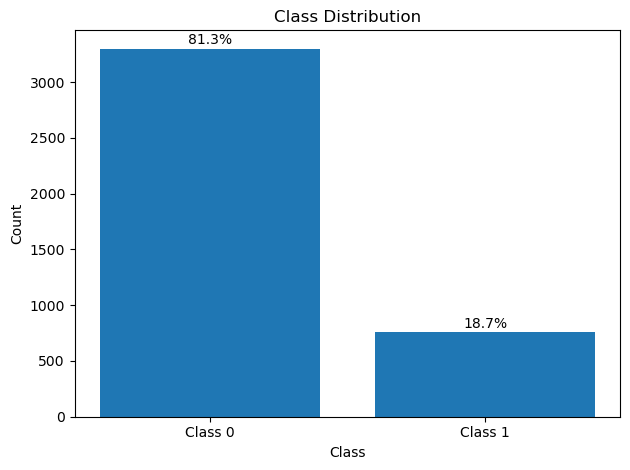
\includegraphics[width=0.5\textwidth]{figures/win_gru_distribution.png}
    \caption{Class distribution after applying window-based filtering in GRU training data. Class 1 increases from 0.02\% to 18.7\%.}
    \label{fig:win-gru-distribution}
\end{figure}

\begin{figure}[H]
    \centering
    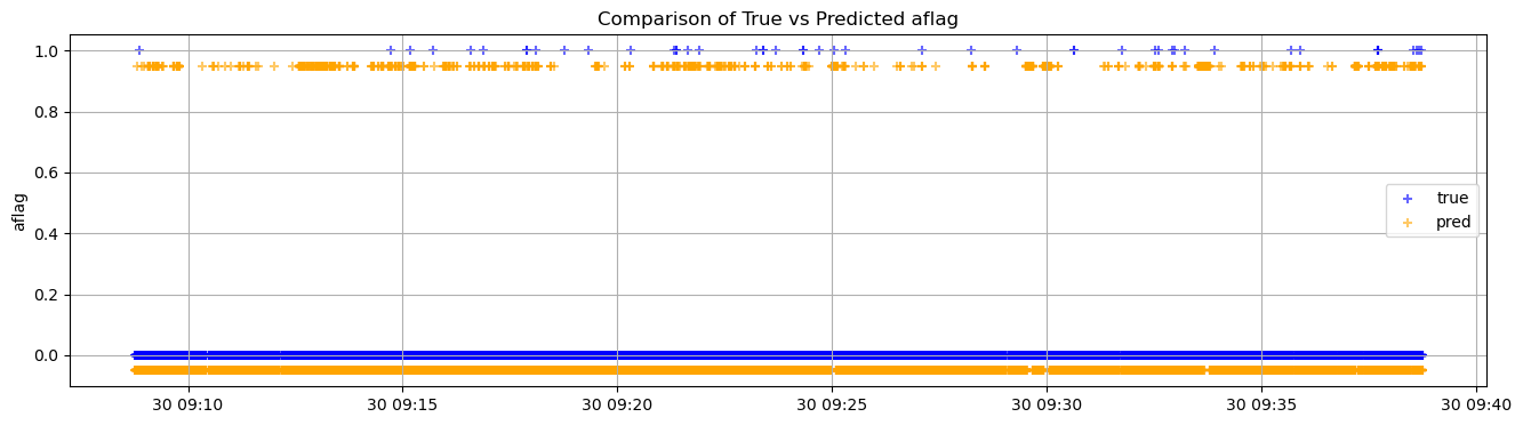
\includegraphics[width=\textwidth]{figures/win_gru_pred_vs_true.png}
    \caption{Window-based GRU: comparison of predicted and true $\bar{\alpha}$. Prediction shifted -0.5 for visibility.}
    \label{fig:win-gru-pred-vs-true}
\end{figure}

\begin{table}[H]
    \centering
    \caption{Confusion matrix and classification report of window-based GRU}
    \label{tab:win-gru-metrics}
    \begin{tabular}{lccc}
        \toprule
        Class & Precision & Recall & F1-score\\
        \midrule
        1 & 0.0146 & 0.4792 & 0.0283 \\
        \midrule
        \textbf{Confusion Matrix} & \multicolumn{3}{c}{} \\
        \midrule
        & Pred 0 & Pred 1 &  \\
        \midrule
        True 0 & 17246 & 1554 &  \\
        True 1 & 25 & 23 &  \\
        \bottomrule
    \end{tabular}
\end{table}

\newpage

\subsection{Hawkes Stage: Feasibility and Efficiency}
%need to do more explaination to show how the result is interpreable
Directly applying the Hawkes process to the full dataset is very slow. It takes more than 12 hours to run, which is not realistic in trading environments. So here, we only use the filtered test timestamps from the WinGRU stage to do simulation, and estimate the Hawkes parameters based on the KM-XGBoost output, which has high recall. This makes the simulation much faster and also cleaner because we already removed lots of noise in previous steps.

In Figure~\ref{fig:hawkes-simulation}, we can see that the simulated event type distribution and timeline match the original ones quite well. The model keeps the overall shape of trading activity, and the inter-arrival time distribution is also similar between real and simulated. So the simulation is doing a good job in capturing the market flow.

Figure~\ref{fig:hawkes-pred-vs-true} shows the predicted versus true aggressive trades. Again, blue '+' are the ground truth, and orange '+' are predicted, shifted down a bit for easier comparison. The pattern is sparser than WinGRU, but still keeps many correct signals.

Table~\ref{tab:hawkes-metrics} gives the classification result. Now the precision reaches 0.2, which is much better than before. The recall is 0.1667, and F1-score is 0.1818. This shows Hawkes simulation is more conservative, but the predictions it gives are more accurate. So this final stage helps us get high-quality aggressive trade points for analysis or action.

Table~\ref{tab:hawkes-metrics} shows the classification result. Now the precision reaches 0.2, which is much better than before. The recall is 0.1667, and the F1-score is 0.1818. This shows that the Hawkes simulation is more conservative, but the predictions it gives are more accurate. So this final stage helps us get high-quality aggressive trade points which is more reasonable to be applied to FX trading backtesting.

\begin{figure}[H]
    \centering
    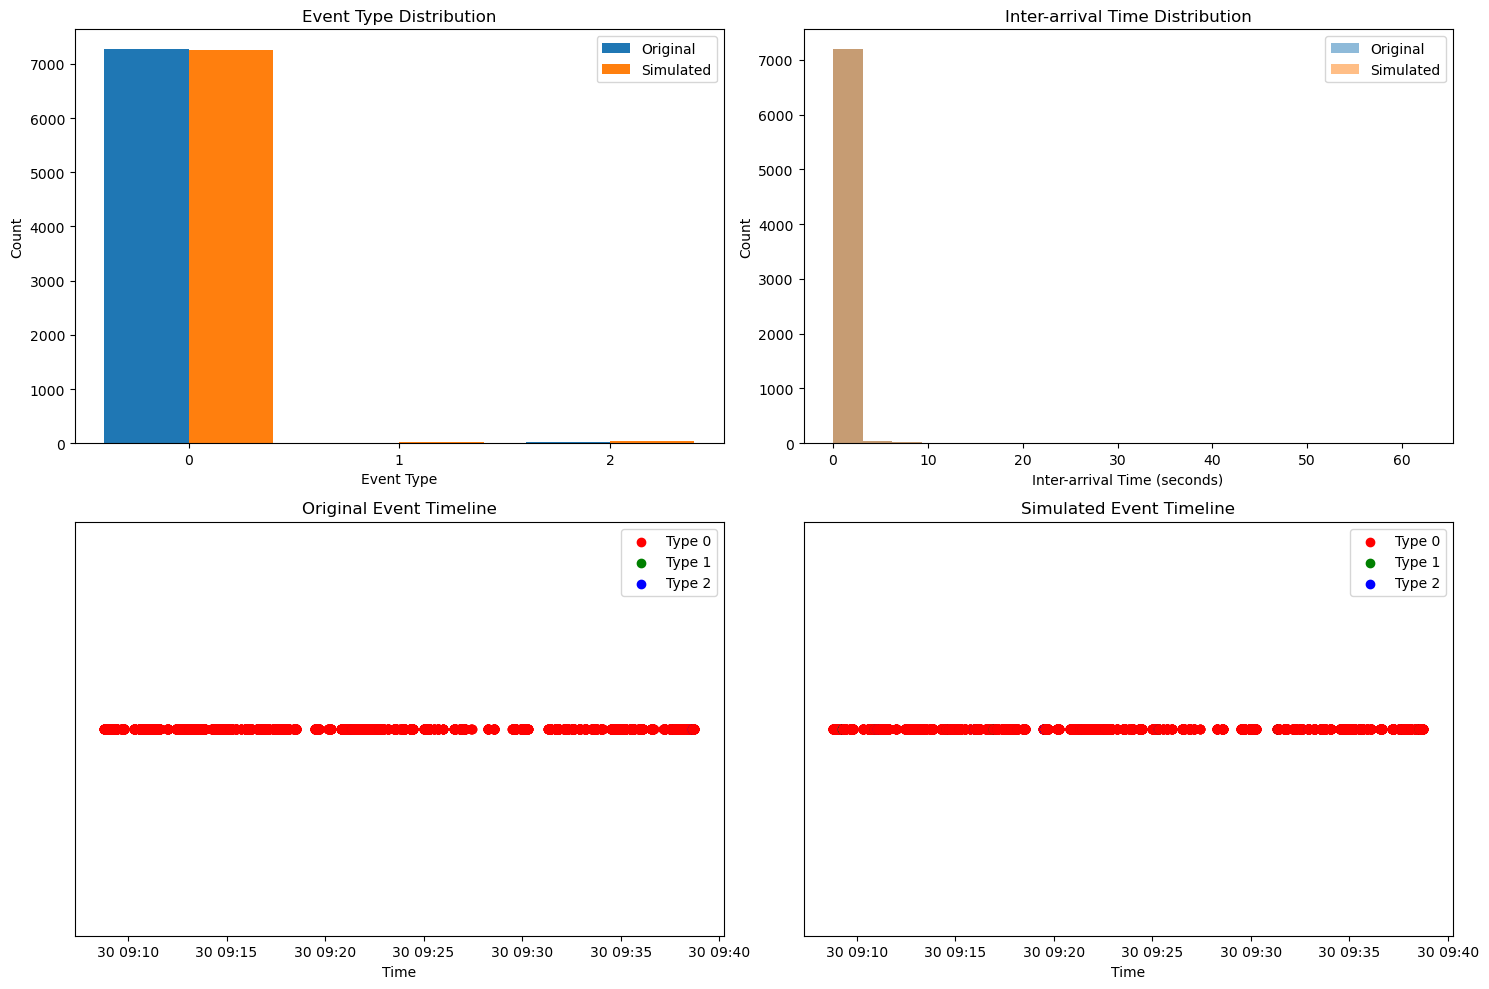
\includegraphics[width=\textwidth]{figures/hawkes_simulation.png}
    \caption{Hawkes process simulation result: event type distribution, inter-arrival time, and timeline comparison.}
    \label{fig:hawkes-simulation}
\end{figure}

\begin{figure}[H]
    \centering
    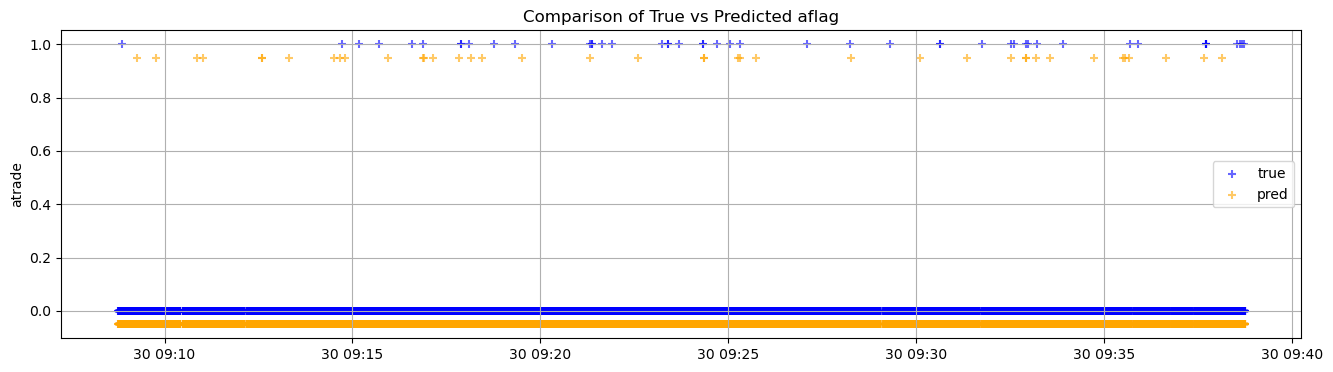
\includegraphics[width=\textwidth]{figures/hawkes_pred_vs_true.png}
    \caption{Comparison of true vs. predicted $\bar{\alpha}$ from Hawkes simulation. Prediction is shifted -0.5 on the y-axis.}
    \label{fig:hawkes-pred-vs-true}
\end{figure}

\begin{table}[H]
    \centering
    \caption{Confusion matrix and classification report of Hawkes simulation}
    \label{tab:hawkes-metrics}
    \begin{tabular}{lccc}
        \toprule
        Class & Precision & Recall & F1-score \\
        \midrule
        1 & 0.2000 & 0.1667 & 0.1818 \\
        \midrule
        \textbf{Confusion Matrix} & \multicolumn{3}{c}{} \\
        \midrule
        & Pred 0 & Pred 1 & \\
        \midrule
        True 0 & 18768 & 32 & \\
        True 1 & 40 & 8 & \\
        \bottomrule
    \end{tabular}
\end{table}

\subsection{Result Conclusion and Data Flow}
\begin{figure}[H]
    \centering
    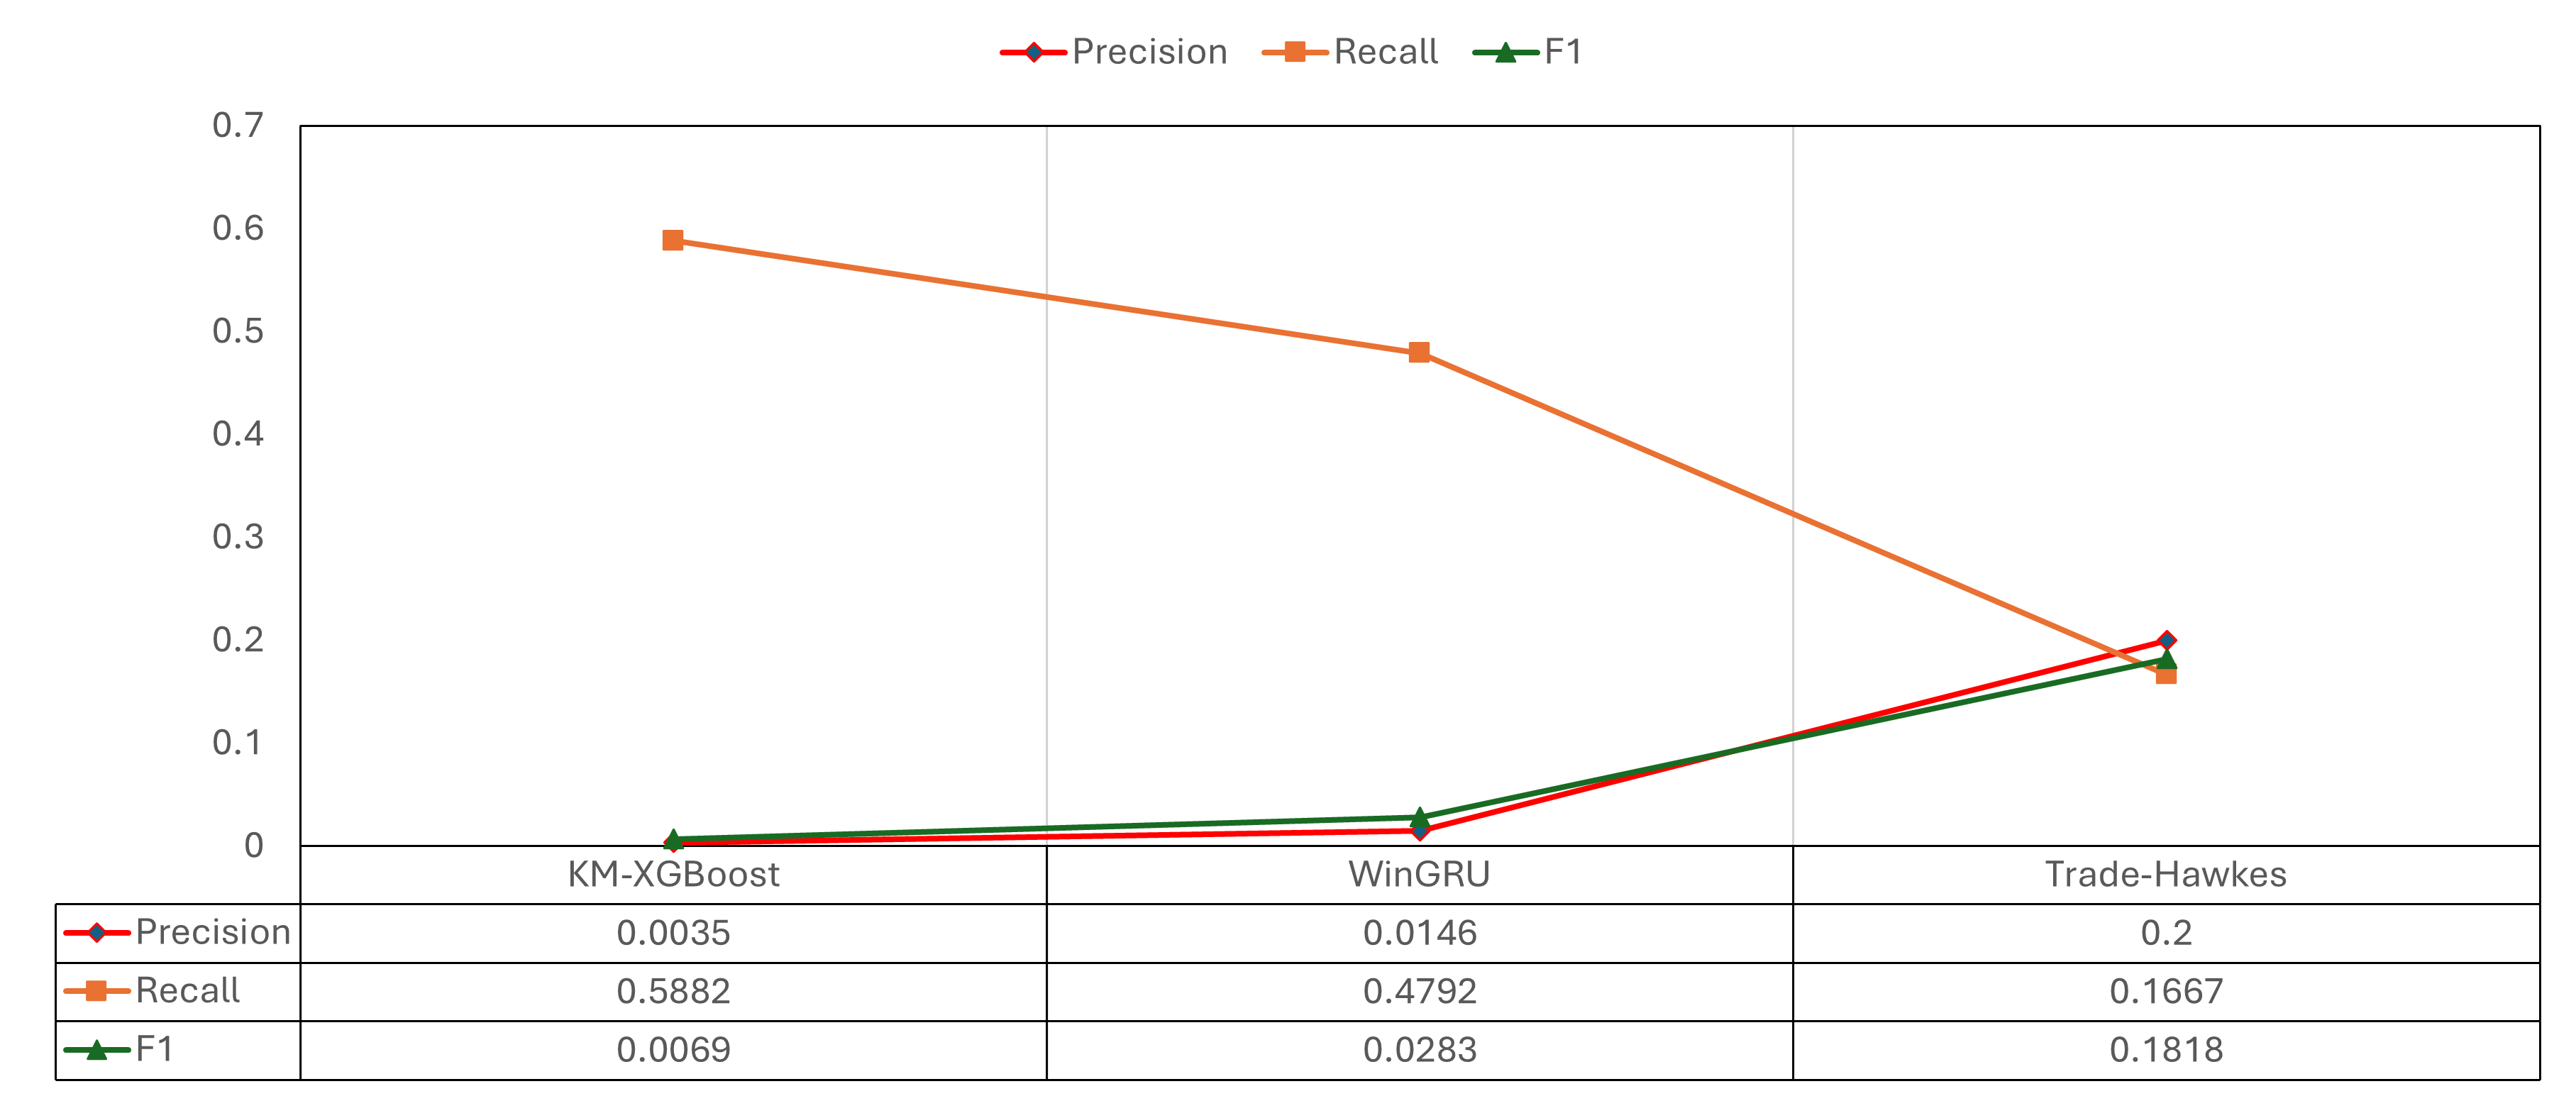
\includegraphics[width=0.9\textwidth]{figures/final_performance_plot.png}
    \caption{Precision, recall, and F1-score across different stages.}
    \label{fig:final-performance}
\end{figure}

\begin{figure}[H]
    \centering
    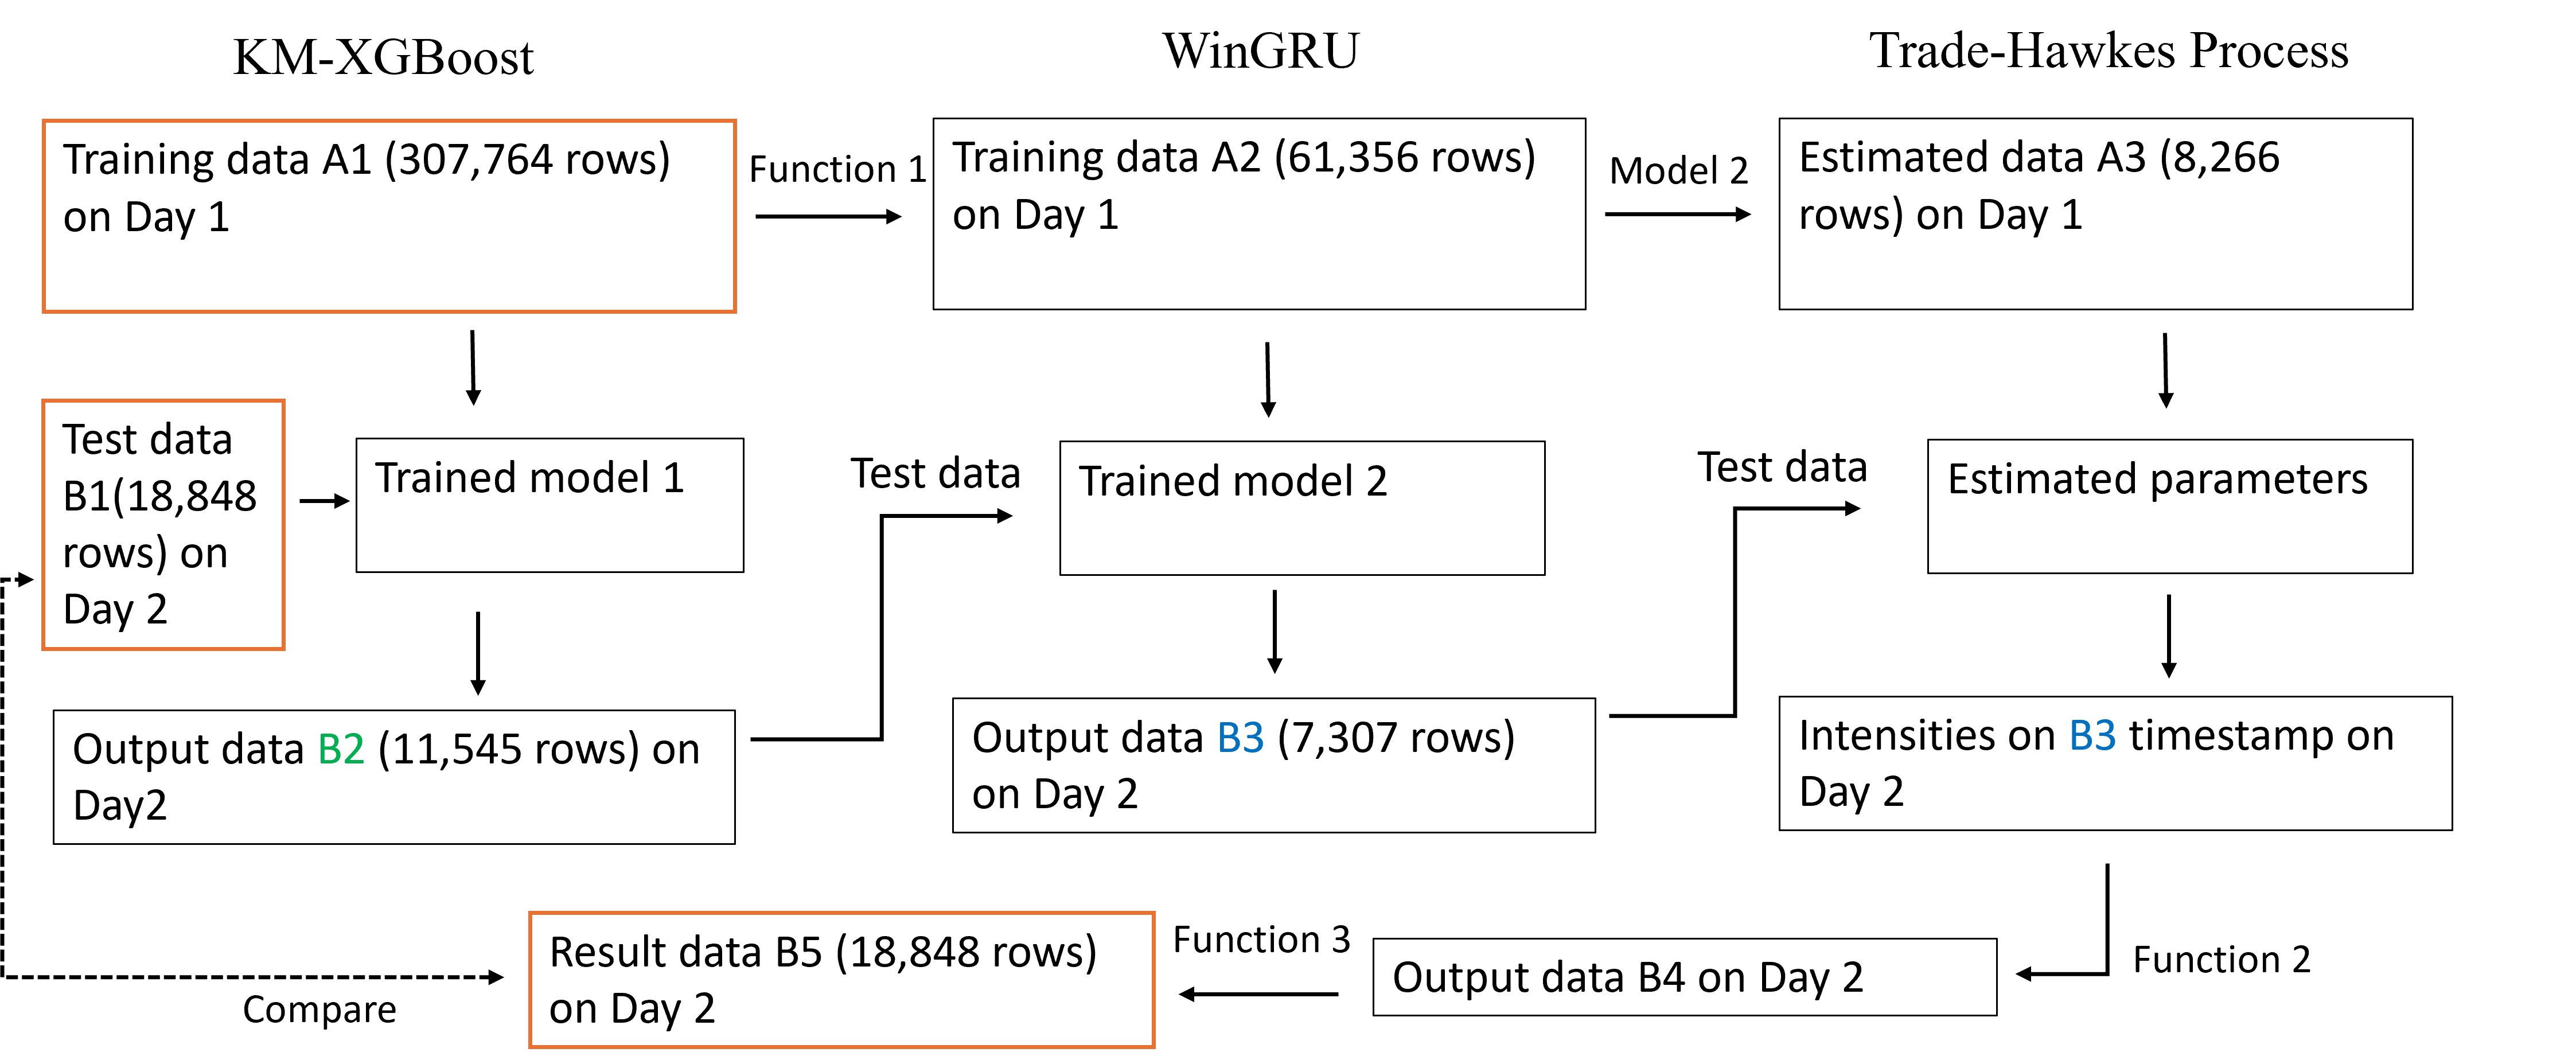
\includegraphics[width=\textwidth]{figures/data flow.png}
    \caption{Data flow of the full pipeline from raw data to final prediction.}
    \label{fig:data-flow-diagram}
\end{figure}

\section{Overall Framework Results}
In this section, we evaluate the performance of the Two-stage Machine Learning and Stochastic Modeling Framework on different trading days, including. The results are compared against several single-model benchmark models, such as only XGBoost, only GRU and Hawkes process. This comparison demonstrates the accuracy and effectiveness of the combined framework in improving simulation performance, particularly under extreme class imbalance.













% \section{Prediction for $\bar{\alpha}$}
% \begin{figure}[h]
%     \centering
%     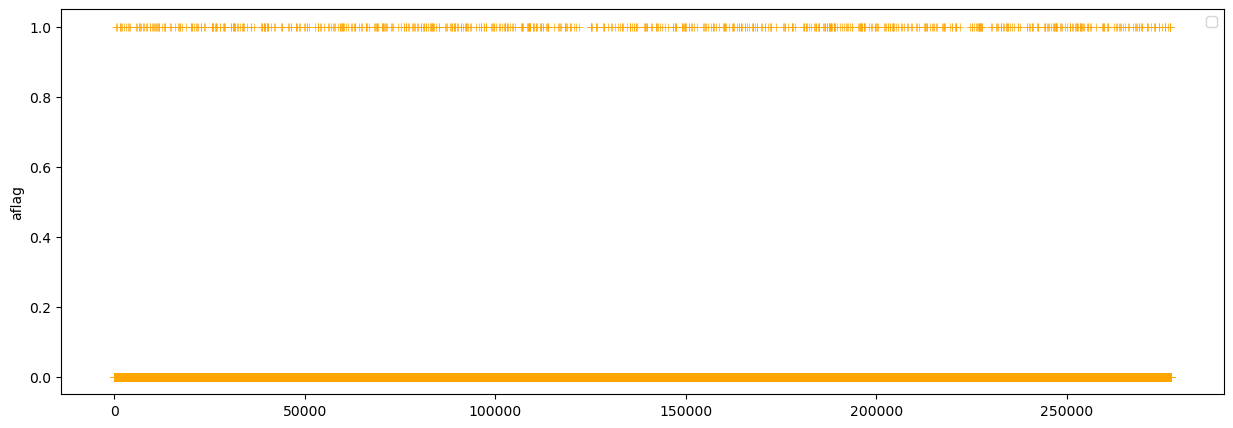
\includegraphics[width=\linewidth]{figures/aflag.png}
%     \caption{Binary distribution of the aggressive trade flag $\bar{\alpha}$}
%     \label{fig: aflag}
%     {\small \textit{Note.} Each point with value 1 indicates the occurrence of an aggressive trade, while 0 indicates non-aggressive or no trade.}
% \end{figure}
% Figure.~\ref{fig: aflag_class_distribution} shows $\bar{\alpha}$ faces severe class imbalance, which can lead to biased model predictions if not addressed. Class 0 dominates the dataset, accounting for 99.8\% of all samples, while Class 1 accounts for only 0.2\%. To solve this imbalance, techniques such as resampling, weighted loss functions, and anomaly detection methods are employed. 
% \begin{figure}[h]
%     \centering
%     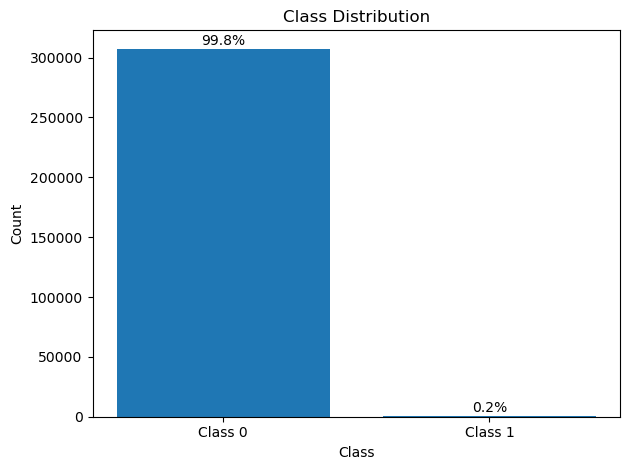
\includegraphics[width=0.8\linewidth]{figures/Imbalaced data for aflag.png}
%     \caption{Class Distribution for $\bar{\alpha}$}
%     {\small \textit{Note.} In the overall 308,178 data, class 0 accounts for 99.8\% of the samples, while Class 1 represents only 0.2\%, indicating a severe class imbalance.}
%     \label{fig: aflag_class_distribution}
% \end{figure}
% \newpage
% \subsection{XGBoost}
% \begin{figure}[h]
%     \centering
%     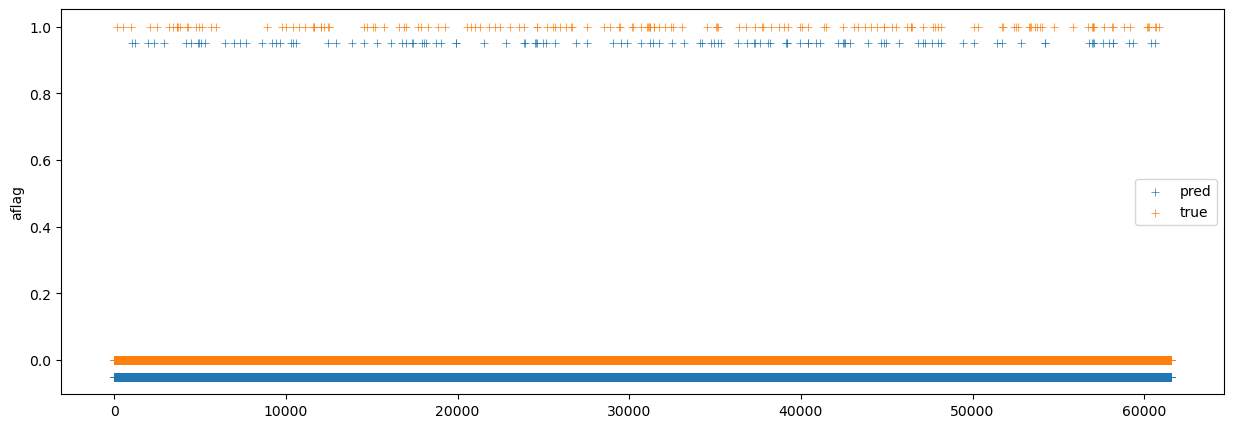
\includegraphics[width=\linewidth]{figures/aflag_XGBoost.png}
%     \caption{Predicted and true values of $\bar{\alpha}$}
%     \label{fig:aggressive_flag_prediction}
%     {\small \textit{Note.} The plot compares the predicted and true values of the aggressive flag. Each `+` marker represents a positive prediction (blue) or ground truth (orange). The strong class imbalance and sparsity of positive cases make correct prediction more difficult, highlighting the challenge of this classification task.}
% \end{figure}
% The model's performance on the test set is summarized by the confusion matrix and associated classification metrics. 

% \begin{table}[h]
% \centering
% \caption{Confusion Matrix}
% \begin{tabular}{c|cc}
% \toprule
%               & Predicted 0 & Predicted 1 \\
% \midrule
% Actual 0      & 61311       & 99          \\
% Actual 1      & 136         & 17          \\
% \bottomrule
% \end{tabular}
% \label{tab:confusion_matrix}
% \vspace{2mm}

% {\small \textit{Note.} The confusion matrix shows a strong true negative rate but a weak true positive rate, which is expected in highly imbalanced classification tasks.}
% \end{table}

% \begin{table}[h]
% \centering
% \caption{Classification Report}
% \begin{tabular}{lcccc}
% \toprule
% Class & Precision & Recall & F1-score & Support \\
% \midrule
% 0     & 0.9978    & 0.9984 & 0.9981   & 61410   \\
% 1     & 0.1466    & 0.1111 & 0.1264   & 153     \\
% \midrule
% Accuracy     & \multicolumn{3}{c}{0.9962} & 61563 \\
% Macro Avg    & 0.5722 & 0.5547 & 0.5622   & 61563 \\
% Weighted Avg & 0.9957 & 0.9962 & 0.9959   & 61563 \\
% \bottomrule
% \end{tabular}
% \label{tab:classification_report}
% \vspace{2mm}

% {\small \textit{Note.} While the overall accuracy is high due to the dominance of class 0, the metrics for class 1 reveal the difficulty of detecting aggressive trades.}
% \end{table}

% \noindent
% \textbf{AUC:} 0.6424
% {\small \textit{Note.} The Area Under the Curve (AUC) score indicates the ability to separate the two classes.}

% \subsection{Feature Importance}
% \begin{figure}[h]
%     \centering
%     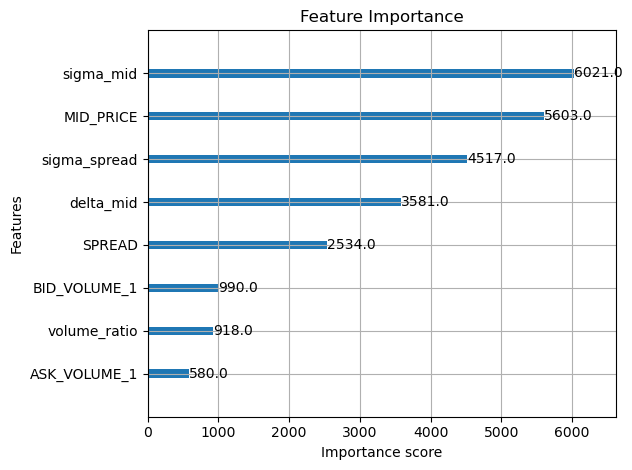
\includegraphics[width=\linewidth]{figures/feature importance.png}
%     \caption{Feature importance scores for predicting aggressive trades}
%     \label{fig:feature_importance_af}
%     {\small \textit{Note.} The most important features include \texttt{sigma\_mid}, \texttt{MID\_PRICE}, and \texttt{sigma\_spread}, indicating that mid-price volatility and spread dynamics play a key role in identifying aggressive trade behavior. Volume-related features such as \texttt{ASK\_VOLUME\_1} and \texttt{BID\_VOLUME\_1} are less influential.}
% \end{figure}

% \newpage


% \section{Prediction for $\alpha$}
% \begin{figure}[h]
%     \centering
%     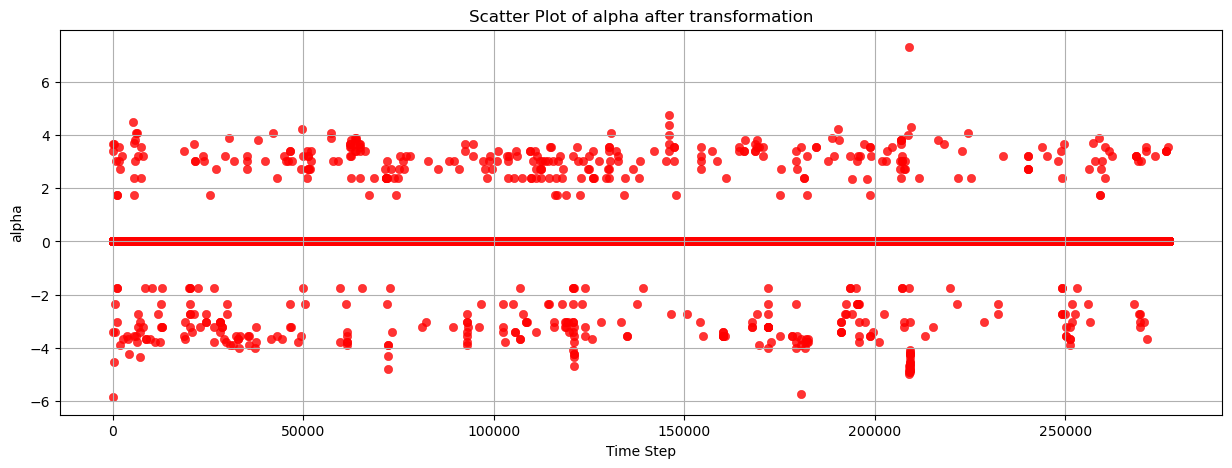
\includegraphics[width=\linewidth]{figures/alpha after transformation.png}
%     \caption{Scatter plot of transformed $\alpha$ values over time}
%     \label{fig:alpha_transformed_scatter}
%     {\small \textit{Note.} This plot visualizes the transformed $\alpha$ signal across time steps. Most values are concentrated near zero, while some are clearly positive or negative.}
% \end{figure}
% \subsection{GRU-based Neural Network}
% \begin{figure}[h]
%     \centering
%     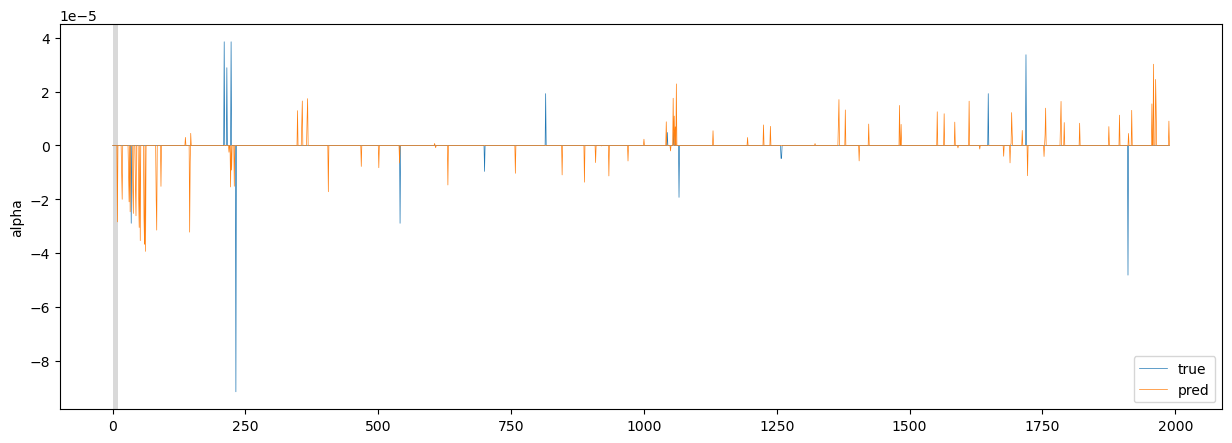
\includegraphics[width=\linewidth]{figures/alpha_GRU.png}
%     \caption{Prediction of $\alpha$ using a GRU-based model}
%     \label{fig:gru_alpha_prediction}
%     {\small \textit{Note.} This plot compares the predicted $\alpha$ values from a GRU model (orange) against the ground truth (blue). The GRU captures some local patterns.}
% \end{figure}
% \begin{figure}[h]
%     \centering
%     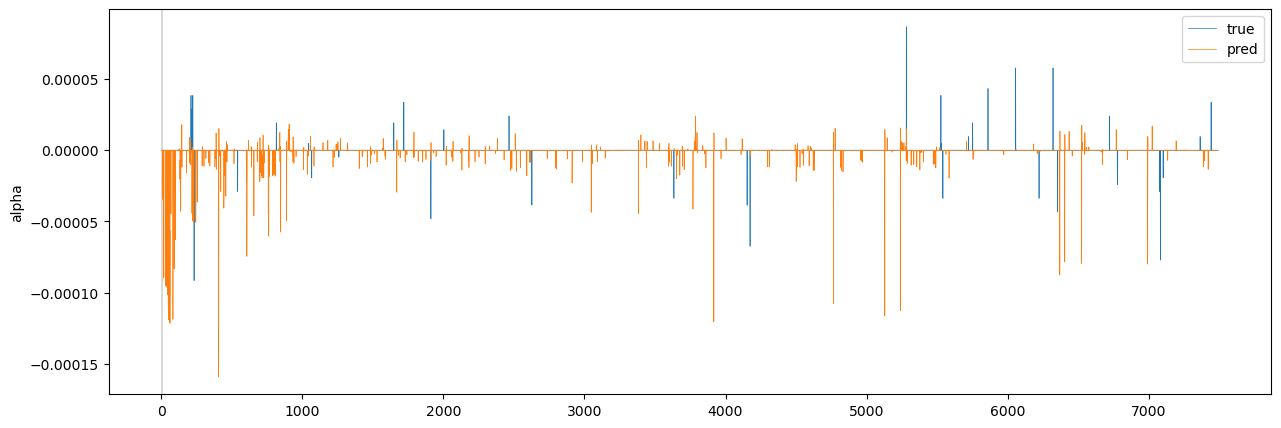
\includegraphics[width=\linewidth]{figures/alpha_Linear.png}
%     \caption{Prediction of $\alpha$ using a linear regression model}
%     \label{fig:lr_alpha_prediction}
%     {\small \textit{Note.} The linear regression model shows limited ability to capture fluctuations in $\alpha$, often underestimating both amplitude and timing compared to the true values. This highlights the limitations of linear models in capturing non-linear temporal dependencies.}
% \end{figure}

% \begin{table}[h]
%     \centering
%     \caption{Performance comparison between GRU and Linear Regression for $\alpha$ prediction}
%     \label{tab:gru_vs_lr}
%     \begin{tabular}{lcc}
%         \toprule
%         Metric & GRU & Linear Regression \\
%         \midrule
%         MSE   & 0.1348  & 0.3336 \\
%         RMSE  & 0.3672  & 0.5776 \\
%         MAE   & 0.0263  & 0.0367 \\
%         %R$^2$ & 3.1362  & 21.0387 \\
%         MAPE (\%) & 63.47  & 62.74 \\
%         SMAPE (\%) & 59.95  & 62.11 \\
%         \bottomrule
%     \end{tabular}
% \end{table}
% Table~\ref{tab:gru_vs_lr} compares the performance of the GRU model and the linear regression model on the task of predicting $\alpha$. The GRU model achieves lower MSE (0.1348 vs. 0.3336), RMSE (0.3672 vs. 0.5776), and MAE (0.0263 vs. 0.0367), indicating better overall prediction accuracy. Although both models show similar MAPE and SMAPE values, the GRU produces a slightly lower symmetric error. 
% % The R$^2$ values are unusually high for both models, likely due to the small magnitude of $\alpha$ and possible data scaling effects, but the relative comparison still shows the GRU outperforming the linear model. 
% Overall, the GRU model demonstrates better capability in capturing the temporal and nonlinear dynamics of the data.

% \section{Prediction for $\tau$}
% Figure.~\ref{fig: Countdown} shows how much time is left until the next aggressive trade. Each point at 0 represents for an aggressive trade. After each zero point, a sharp increase marks the start of a new countdown period leading up to the next aggressive trade.
% \begin{figure}[h]
%     \centering
%     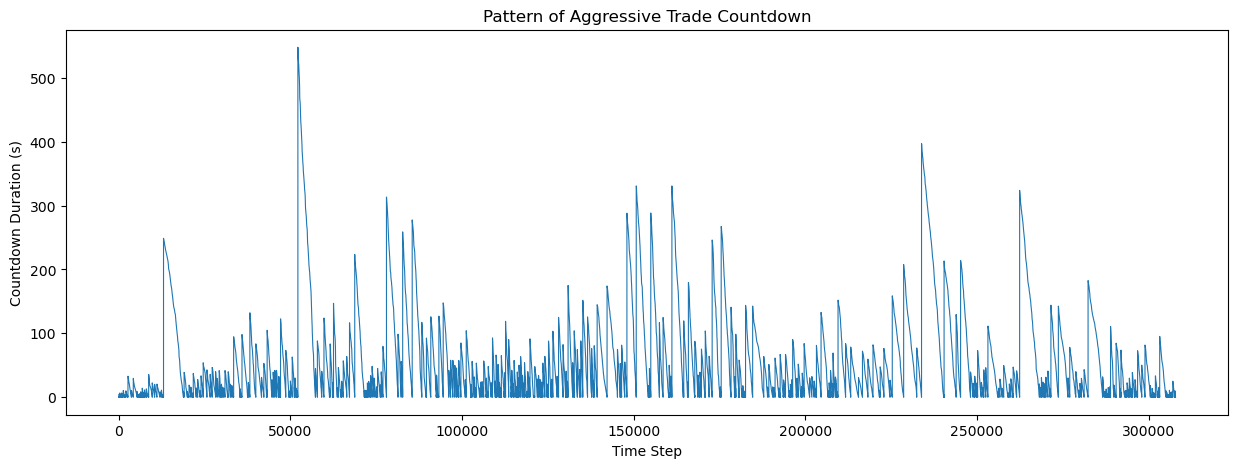
\includegraphics[width=\linewidth]{figures/Pattern of Aggressive Trade Countdown.png}
%     \caption{Countdown to the next aggressive trade}
%     \label{fig: Countdown}
% \end{figure}

% \subsection{XGBoost}
% \subsection{Recurrent Neural Networks}
% The feature matrix $X$ and the target vector $y$ are converted to NumPy arrays. The dataset is split into training (90\%) and testing (10\%) sets. Both the input and output are scaled to improve convergence during training. Inputs are normalized to the range $[0, 1]$ using a MinMaxScaler. For the output, to enhance the sensitivity of the model to small but informative signals, we applied a signed logarithmic transformation to selected features. The transformation preserves the original sign of the data, compresses large magnitudes, and expands small nonzero values, making subtle patterns more noticeable to the model. After applying the logarithmic adjustment, the transformed values are rescaled to fit within the range \([-1, 1]\). An inverse transformation is also defined to recover the original values when necessary, maintaining consistency between the transformed and original feature spaces.


% \section{Ablation Studies}
% Impact of different model components (CGAN vs. pure Hawkes vs. hybrid). Sensitivity analysis on model hyperparameters.


% \section{Backtesting Performance}
% Simulating market impact with aggressive/passive execution strategies.
% Evaluating execution cost and slippage in various market scenarios.
% Comparing execution performance with traditional historical replay.

% \section{Application to other products}
% other products, like FX options, equity...